\documentclass[11pt,a4paper]{article}
\usepackage{fontspec}
\usepackage{polyglossia}
\setmainlanguage{turkish}
\setotherlanguage{english}
\setmainfont{TeX Gyre Termes}
\usepackage{amsmath,amssymb}
\usepackage[margin=2.3cm]{geometry}
\usepackage{graphicx}
\usepackage{booktabs}
\usepackage{multirow}
\usepackage{array}
\usepackage{tabularx}
\usepackage{caption}
\usepackage{subcaption}
\usepackage{xcolor}
\usepackage{tikz}
\usetikzlibrary{arrows.meta,positioning,fit,calc}
\usepackage{amsthm}
\usepackage{enumitem}
\usepackage{microtype}
\usepackage{flafter}
\usepackage[hidelinks]{hyperref}
\usepackage{cite}

\captionsetup{font=small,labelfont=bf,labelsep=period}
\setlength{\parskip}{0.25em}
\setlength{\emergencystretch}{1.5em}
\setlist{itemsep=0.15em,topsep=0.3em}
\renewcommand{\topfraction}{0.95}
\renewcommand{\textfraction}{0.05}
\renewcommand{\floatpagefraction}{0.85}
\setcounter{topnumber}{3}
\setcounter{totalnumber}{4}
\makeatletter
\renewcommand{\fps@figure}{t}
\renewcommand{\fps@table}{t}
\makeatother

\newtheorem{proposition}{Önerme}
\theoremstyle{definition}
\newtheorem{definition}{Tanım}

\newcommand{\Luk}{\mathrm{L}}
\newcommand{\osfis}{OSFI-DJ-S}
\newcommand{\osfins}{OSFI-DJ-NS}

\title{\textbf{İzole Kavşakta Trafik Sinyali Kontrolü için Benzerlik Optimizasyonlu Bulanık Çıkarım (OSFI): Yeniden Gerçekleştirme ve Sensör Gürültüsüne Dayanıklı Non-Singleton Genişletme}}
\author{Ömer Faruk İşcanlı\\[0.2em]
\small Bilgisayar Mühendisliği, İstanbul Üniversitesi-Cerrahpaşa\\
\small Öğrenci No: 1306220071\\[0.2em]
\small Bulanık Mantık Dersi Dönem Projesi --- Prof. Dr. Rüya Şamlı\\
\small Kod deposu: \url{https://github.com/iscanliomerfaruk/osfi-traffic-signal-control}}
\date{16 Kasım 2026}

\begin{document}
\maketitle

\begin{abstract}
\noindent Bu çalışmada Esmaeili vd.~\cite{esmaeili2025osfi} tarafından önerilen, izole bir kavşakta yeşil süre uzatmasını iki aşamalı bir bulanık kontrolcüyle belirleyen \emph{Optimization Similarity Fuzzy Inference} (OSFI) yöntemi incelenmiş, açık kaynaklı bir Python simülatörü üzerinde yeniden gerçekleştirilmiş ve genişletilmiştir. Referans makalede eksik bırakılan 23 kural, üyelik fonksiyonu parametreleri ve faz geçiş mantığı belgelenmiş varsayımlarla tamamlanmış; yöntem hem makalede yazıldığı biçimiyle (OSFI-literal) hem de Deng ve Jiang'ın~\cite{deng2014osfi} doğruluk tablosu benzerliği optimizasyonuna sadık biçimiyle (OSFI-DJ) kodlanmıştır. Teorik katkı olarak, tekil (singleton) bulanıklaştırma altında $d_1$ benzerliğine dayalı OSFI çözümünün kapalı biçimde $B^*(y)=I(A(x_0),B(y))$'ye, yani aynı implikatörle kurulan kompozisyonel çıkarım kuralına (CRI) indirgendiği gösterilmiş ve 30 tohumluk deneylerde birebir doğrulanmıştır. Bu sonuçtan hareketle, OSFI'nin klasik çıkarımdan ancak tekil olmayan (non-singleton) girişlerde ayrışabildiği gözlemlenmiş ve gürültülü kuyruk/varış sensörleri için eşleştirilmiş Gauss bulanıklaştırmalı bir non-singleton OSFI (\osfins) önerilmiştir. Kontrollü deneylerde Łukasiewicz implikatörlü OSFI-DJ, ağır trafikte gecikmeyi Mamdani'ye göre \%5,9, Sugeno'ya göre \%46 azaltmış; makalede yazıldığı biçimdeki OSFI-literal ise Mamdani'nin gerisinde kalmıştır. \osfins, düşük--orta gürültüde (σ$_q\le5$ m) tekil OSFI'ye göre \%1--4 ek iyileşme sağlamış, yüksek gürültüde fark istatistiksel olarak anlamlı bulunmamıştır. Ayrıca Łukasiewicz VE işlecinin makaledeki Gauss üyelik fonksiyonlarıyla giriş uzayının \%5'inde hiçbir kuralın ateşlenmediği ``ölü bölgeler'' oluşturduğu tespit edilmiştir.

\smallskip\noindent\textbf{Anahtar kelimeler:} bulanık çıkarım, trafik sinyali kontrolü, OSFI, kompozisyonel çıkarım kuralı, non-singleton bulanıklaştırma, Łukasiewicz t-normu
\end{abstract}

\section{Giriş}
\label{sec:intro}

Kentsel kavşaklardaki gecikme, yakıt tüketimi ve emisyonun önemli bir kaynağıdır. Sabit zamanlı planlar (ör. Webster~\cite{webster1958}) ortalama talebe göre tasarlandığından anlık dalgalanmalara uyum sağlayamaz; araç uyarmalı kontrol ise basit eşik kurallarına dayanır~\cite{eom2020}. Bulanık mantık, ``kuyruk uzun'', ``varış hızı yüksek'' gibi dilsel ifadeleri doğrudan kural tabanına taşıyarak uzman bilgisini kontrol yasasına çevirmeyi sağlar ve trafik sinyali kontrolünde Pappis ve Mamdani'nin öncü çalışmasından~\cite{pappis1977} bu yana yaygın biçimde kullanılmaktadır.

Esmaeili vd.~\cite{esmaeili2025osfi}, Deng ve Jiang'ın doğruluk tablosu benzerliğini optimize eden çıkarım yöntemini~\cite{deng2014osfi} trafik sinyali kontrolüne uyarlayan OSFI yöntemini önermiş ve Mamdani ile Sugeno kontrolcülerine göre gecikmede \%0,7--5,7 iyileşme bildirmiştir. Ancak makalede kural tabanlarının çoğu, simülasyon parametreleri ve OSFI optimizasyonunun nasıl çözüldüğü verilmemiştir. Bu durum, yöntemin bağımsız olarak doğrulanmasını zorlaştırmaktadır.

Bu projenin amacı (i) referans yöntemi bilimsel ve teknik açıdan incelemek, (ii) yeniden üretilebilir bir uygulamasını oluşturmak, (iii) yöntem üzerinde ölçülebilir bir katkı geliştirmek ve (iv) sonuçları kontrollü, istatistiksel olarak değerlendirilmiş deneylerle karşılaştırmaktır. Katkılar şunlardır:
\begin{enumerate}
\item NPS--GPE--SPM mimarisinin, beş çıkarım motorunun (Mamdani, Sugeno, OSFI-literal, OSFI-DJ, CRI) ve iki klasik karşılaştırma yönteminin (Webster, araç uyarmalı) sıfırdan, harici bulanık mantık kütüphanesi kullanılmadan Python ile gerçekleştirilmesi ve tüm varsayımların belgelenmesi.
\item Tekil bulanıklaştırma altında $d_1$-OSFI'nin CRI'ya indirgendiğini gösteren bir önerme ve bunun sayısal olarak doğrulanması (Bölüm~\ref{sec:prop}).
\item Sensör gürültüsüne karşı eşleştirilmiş Gauss bulanıklaştırmalı non-singleton OSFI ve bu katkının kaynağını ayrıştırmak için non-singleton CRI kontrol koşulu (Bölüm~\ref{sec:ext}).
\item 30 ortak rastgele sayı tohumu, \%95 güven aralıkları, Wilcoxon işaretli sıra testi ve Holm düzeltmesiyle yürütülen karşılaştırmalı deneyler, ablasyon çalışması ve Łukasiewicz VE işlecinden kaynaklanan ölü bölgelerin tanılanması.
\end{enumerate}

\section{İlgili Çalışmalar}
\label{sec:related}

\textbf{Klasik bulanık sinyal kontrolü.} Pappis ve Mamdani~\cite{pappis1977}, tek kavşakta yeşil uzatma kararını bulanık kurallarla veren ilk kontrolcüyü önermiştir. Trabia vd.~\cite{trabia1999}, yaklaşım akışlarından trafik yoğunluğunu kestiren ve ikinci aşamada fazın uzatılıp sonlandırılacağına karar veren iki aşamalı bir yapı tanımlamıştır. Referans makaledeki FC$_1$/FC$_2$ ayrımı bu yapıya kavramsal olarak çok yakındır. Niittymäki ve Pursula~\cite{niittymaki2000} ile Murat ve Gedizlioglu~\cite{murat2005}, çok fazlı izole kavşaklarda bulanık faz sıralaması ve uzatma kararlarını incelemiştir.

\textbf{Optimizasyonla ayarlanan ve Tip-2 bulanık kontrolcüler.} Bi vd., diferansiyel evrimle ayarlanan Tip-2 bulanık çoklu kavşak kontrolü~\cite{bi2014} ve arter koordinasyonu için optimal Tip-2 sistem~\cite{bi2018} önermiştir. Lin vd.~\cite{lin2023} bulanık kontrolü diferansiyel evrimle, Korkmaz ve Akgüngör~\cite{korkmaz2024} Tip-2 bulanık mantığı çiçek tozlaşma ve karga arama algoritmalarıyla birleştirmiştir. Jovanović vd.~\cite{jovanovic2023} aralık Tip-2 bulanık mantığı kısıtlı U-dönüşlü kavşaklara uygulamıştır. Chala ve Kóczy~\cite{chala2024}, kuyruk değerlendirmesi, yoğunluk tespiti ve acil araç önceliğini birleştiren üç aşamalı hiyerarşik bir bulanık kontrolcü sunmuş ve gömülü sensörlerin kuyruğun tamamını göremediğini vurgulamıştır. Ali vd.~\cite{ali2021} bulanık kontrolü Webster formülüyle birleştirerek SUMO'da değerlendirmiştir.

\textbf{Öğrenme tabanlı hibrit yöntemler.} Kumar vd.~\cite{kumar2021} ve Tunc ile Soylemez~\cite{tunc2023} bulanık çıkarımı derin Q-öğrenme ile birleştirmiştir. Bi vd.~\cite{bi2024electronics}, Tip-2 bulanık sistemin çıktısını DQN hedef ağındaki maksimum işleminin yerine kullanmıştır. FuzzyLight~\cite{li2025fuzzylight}, gerçek şehir dağıtımında sensör gürültüsünü bulanık mantık ve sıkıştırılmış algılama ile azaltmayı hedeflemiştir. Bu son çalışma, sensör belirsizliğinin pratik kontrolcüler için temel bir sorun olduğunu göstermesi bakımından bu projenin katkısıyla doğrudan ilişkilidir.

\textbf{Benzerlik tabanlı çıkarım ve non-singleton bulanık sistemler.} Benzerliğe dayalı çıkarım, Zadeh'in kompozisyonel çıkarım kuralına (CRI)~\cite{zadeh1973} alternatif olarak geliştirilmiştir~\cite{wang2008}. Deng ve Jiang~\cite{deng2014osfi} sonucu, kural ile gözlem arasındaki doğruluk tablosu benzerliğini maksimize eden bulanık küme olarak tanımlamış ve çözümün tek olmayabileceğini tartışmıştır. Yöntem sezgisel bulanık kümelere genişletilmiştir~\cite{esmaeili2019}. Mouzouris ve Mendel~\cite{mouzouris1997}, ölçüm gürültüsünü giriş kümesine taşıyan non-singleton bulanık sistemlerin kuramını kurmuş ve gürültülü zaman serilerinde tekil sistemlerden daha iyi sonuç verdiğini göstermiştir. Tablo~\ref{tab:lit}, incelenen başlıca çalışmaları karşılaştırmaktadır. Bildiğimiz kadarıyla OSFI'nin non-singleton girişlerle trafik kontrolüne uygulanması ve CRI ile denkliğinin incelenmesi literatürde yer almamaktadır.

\begin{table}[t]
\centering
\caption{İncelenen başlıca çalışmaların karşılaştırması.}
\label{tab:lit}
\small
\begin{tabularx}{\textwidth}{@{}p{3.1cm}p{3.6cm}X@{}}
\toprule
Çalışma & Yöntem & Bu projeyle ilişkisi \\
\midrule
Pappis, Mamdani~\cite{pappis1977} & Mamdani, tek kavşak & Bulanık yeşil uzatma fikrinin temeli \\
Trabia vd.~\cite{trabia1999} & İki aşamalı bulanık karar & FC$_1$/FC$_2$ yapısının öncülü \\
Bi vd.~\cite{bi2014,bi2018} & Tip-2 + evrimsel ayar & Belirsizliği küme biçiminde modelleme \\
Lin vd.~\cite{lin2023}; Korkmaz, Akgüngör~\cite{korkmaz2024} & Bulanık + meta-sezgisel & Parametre ayarına dayalı iyileştirme \\
Chala, Kóczy~\cite{chala2024} & Üç aşamalı hiyerarşik bulanık & Sensörün kuyruğu kısmen görmesi sorunu \\
Kumar vd.~\cite{kumar2021}; Bi vd.~\cite{bi2024electronics} & Bulanık + derin RL & Öğrenme tabanlı hibrit eğilim \\
FuzzyLight~\cite{li2025fuzzylight} & Bulanık + sıkıştırılmış algılama + RL & Sensör gürültüsüne dayanıklılık \\
Deng, Jiang~\cite{deng2014osfi} & Doğruluk tablosu benzerliği & OSFI'nin kuramsal temeli \\
Mouzouris, Mendel~\cite{mouzouris1997} & Non-singleton bulanık sistem & Önerilen genişletmenin temeli \\
Esmaeili vd.~\cite{esmaeili2025osfi} & OSFI, NPS--GPE--SPM & Referans çalışma \\
\bottomrule
\end{tabularx}
\end{table}

\section{Teorik Altyapı}
\label{sec:theory}

\textbf{Bulanık küme ve dilsel değişken.} $X$ evreni üzerindeki bir bulanık küme $A$, $\mu_A:X\to[0,1]$ üyelik fonksiyonuyla tanımlanır~\cite{zadeh1965}. Dilsel değişken (ör. ``kuyruk uzunluğu''), terimleri (Kısa, Orta, Uzun, Çok Uzun) bulanık kümelerle temsil edilen değişkendir. Bu çalışmada Gauss $\mu(x)=\exp(-(x-c)^2/2\sigma^2)$ ve üçgen üyelik fonksiyonları kullanılmıştır.

\textbf{T-normlar ve implikatörler.} Kural öncüllerindeki VE işlemi bir t-norm ile yapılır: minimum $T_M(a,b)=\min(a,b)$, çarpım $T_P=ab$ ve Łukasiewicz $T_\Luk(a,b)=\max(0,a+b-1)$. Bir bulanık implikatör $I:[0,1]^2\to[0,1]$; $I(0,0)=I(0,1)=I(1,1)=1$ ve $I(1,0)=0$ sınır koşullarını sağlar~\cite{deng2014osfi}. Łukasiewicz $I_\Luk(a,b)=\min(1,1-a+b)$, Goguen $I_G(a,b)=1$ ($a\le b$), aksi halde $b/a$ ve Kleene--Dienes $I_{KD}=\max(1-a,b)$ bu koşulları sağlar. Mamdani'nin $\min(a,b)$ işlemi ise $I(0,0)=0$ verdiğinden gerçek bir implikatör değil, bir bağlaçtır (conjunction).

\textbf{CRI, Mamdani ve Sugeno çıkarımı.} ``$A$ ise $B$'' kuralı $R(x,y)=I(A(x),B(y))$ ilişkisiyle temsil edilir. Zadeh'in kompozisyonel çıkarım kuralına göre gözlem $A^*$ için sonuç $B^*(y)=\sup_x T(A^*(x),R(x,y))$'dir~\cite{zadeh1973}. Mamdani çıkarımında~\cite{mamdani1975} kurallar minimumla kırpılır, maksimumla birleştirilir ve ağırlık merkezi (centroid) ile durulaştırılır: $y^*=\int y\,B^*(y)dy/\int B^*(y)dy$. Sıfırıncı dereceden Sugeno (TSK) çıkarımında~\cite{takagi1985} her kuralın sonucu bir sabittir ($z_i$) ve çıkış $\sum\alpha_iz_i/\sum\alpha_i$ ağırlıklı ortalamasıdır.

\textbf{Benzerlik ölçüsü ve OSFI.} Bulanık ilişkiler arasındaki $d_1$ benzerliği $\mathrm{Sim}(R,R^*)=1-\frac{1}{|X||Y|}\sum_{x,y}|R(x,y)-R^*(x,y)|$ ile tanımlanır. Deng ve Jiang'ın yönteminde~\cite{deng2014osfi} sonuç, kural ile gözlemin doğruluk tablolarını en çok benzeştiren kümedir:
\begin{equation}
B^*=\arg\max_{B'}\ \mathrm{Sim}\big(I(A(x),B(y)),\ I(A^*(x),B'(y))\big).
\label{eq:osfi}
\end{equation}

\textbf{Non-singleton bulanıklaştırma.} Tekil bulanıklaştırmada ölçüm $x_0$ yalnızca kendi noktasında 1 üyelikli bir kümeye dönüşür. Non-singleton bulanıklaştırmada ise ölçüm belirsizliği, $x_0$ merkezli ve gürültü düzeyiyle orantılı genişlikte bir küme ile (ör. Gauss) temsil edilir~\cite{mouzouris1997}.

\section{Referans Makalenin Yöntemi}
\label{sec:original}

Referans çalışma~\cite{esmaeili2025osfi}, her yaklaşımın ayrı bir fazda (Doğu, Güney, Batı, Kuzey) yeşil aldığı dört kollu izole bir kavşağı ve her yaklaşımı M/M/1 kuyruğu olarak modeller. Kontrolcü üç modülden oluşur (Şekil~\ref{fig:arch}):
\begin{itemize}
\item \textbf{NPS} (Next Phase Selection): Sıradaki yeşil fazı, en uzun kuyruğa sahip yaklaşım olarak seçer.
\item \textbf{GPE} (Green Phase Extension): İki bulanık kontrolcüyle yeşil uzatma süresini hesaplar. FC$_1$, mevcut fazın varış hızı $\lambda$ (araç/10 s) ve kuyruk uzunluğundan (m) Uzatma$_1$'i 16 kuralla üretir. FC$_2$ ise Uzatma$_1$ ile diğer fazların kuyruk uzunluğundan Uzatma$_2$'yi 13 kuralla üretir.
\item \textbf{SPM} (Switching Phase Module): NPS ve GPE çıktılarına göre faz değişimini uygular.
\end{itemize}
Üyelik fonksiyonları makalenin Şekil 4--7'sinde verilmiştir. $\lambda$ ve kuyruk girişleri için dörder çan biçimli küme, uzatma çıkışı için dört üçgen küme kullanılmıştır. Makalenin 4.1.2.~bölümünde VE işleminin ``Łukasiewicz implikatörü'' ile yapıldığı ve çıkışın $\sum\alpha_iz_i/\sum\alpha_i$ ağırlıklı ortalamasıyla hesaplandığı belirtilmektedir. Deneyler orta ve ağır trafik için MATLAB'da yapılmış, OSFI'nin Mamdani'ye göre gecikmeyi \%1,1--5,7, Sugeno'ya göre \%0,7--4,8 azalttığı ve ağır trafikte araç çıkışını \%18,75'e kadar artırdığı bildirilmiştir.

\begin{figure}[t]
\centering
\resizebox{\textwidth}{!}{%
\begin{tikzpicture}[
  node distance=0.55cm and 0.8cm,
  box/.style={draw, rounded corners=2pt, align=center, font=\small, minimum height=0.95cm, inner sep=4pt},
  arr/.style={-{Stealth[length=2mm]}, semithick}]
\node[box, fill=gray!8] (sens) {Sensörler\\ $\lambda$, $q_E,q_S,q_W,q_N$};
\node[box, fill=blue!7, right=1.0cm of sens, yshift=0.75cm] (fc1) {FC$_1$ (16 kural)\\ $(\lambda,q_{\text{akt}})\to$ Uzatma$_1$};
\node[box, fill=blue!7, right=0.8cm of fc1] (fc2) {FC$_2$ (13 kural)\\ $(\text{Uzatma}_1,q')\to$ Uzatma$_2$};
\node[box, fill=green!7, below=0.55cm of fc1] (nps) {NPS\\ en uzun kuyruk};
\node[box, fill=orange!10, right=0.8cm of fc2, yshift=-0.75cm] (spm) {SPM\\ uzat / fazı değiştir};
\node[box, fill=gray!8, right=0.6cm of spm] (sig) {Sinyal\\ ve kavşak};
\node[draw, dashed, rounded corners, inner sep=5pt, fit=(fc1)(fc2), label={[font=\small]above:GPE}] {};
\draw[arr] (sens) |- (fc1);
\draw[arr] (sens) |- (nps);
\draw[arr] (fc1) -- (fc2);
\draw[arr] (fc2) -| (spm);
\draw[arr] (nps) -| ($(spm.south)+(-0.2,0)$);
\draw[arr] (spm) -- (sig);
\draw[arr] (sig.south) -- ++(0,-1.05) -| (sens.south);
\end{tikzpicture}}
\caption{Referans kontrolcünün NPS--GPE--SPM mimarisi. $q'$, diğer üç fazın kuyruklarının en büyüğüdür (bu projedeki varsayım).}
\label{fig:arch}
\end{figure}

\textbf{Eleştirel değerlendirme.} Makaleyi yeniden gerçekleştirirken doğrudan PDF'e karşı doğrulanan şu sorunlar belirlenmiştir:
\begin{enumerate}[label=(\alph*)]
\item Tablo 1--2'deki ``Average Exit'' iyileşmeleri, daha az araç çıkışını iyileşme sayan bir işaretle hesaplanmıştır (ör. Doğu fazında 328'e karşı 310 araç, ``\%5,49 iyileşme''). Oysa metin, daha yüksek çıkışın daha iyi olduğunu söylemektedir. Ayrıca iki tabloda yüzde paydası farklıdır.
\item Dört fazlı bir sinyalde, en az 7 s'lik yeşil ve kırmızı bekleme süreleri altında ortalama gecikmenin $\approx$1,0--1,2 s/araç olması fiziksel olarak mümkün değildir.
\item OSFI denklem~\eqref{eq:osfi} ile tanımlanmasına rağmen hangi benzerlik ölçüsünün ve implikatörün kullanıldığı ve optimizasyonun nasıl çözüldüğü verilmemiştir. Uygulanan formül Łukasiewicz t-normlu sıfırıncı dereceden bir Sugeno sistemine eşdeğerdir. Öte yandan tüm kontrolcülerde centroid durulaştırma kullanıldığı söylenmektedir.
\item 29 kuralın 23'ü verilmemiş, üyelik fonksiyonu aralıkları metin ile şekiller arasında çelişmektedir. Tekrar sayısı, tohum, talep düzeyi ve istatistiksel test raporlanmamıştır.
\end{enumerate}
Bu nedenle mutlak sayıların birebir yeniden üretilmesi beklenmemiş, karşılaştırma yöntemlerin sıralaması ve göreli farklar üzerinden yapılmıştır.

\section{Yeniden Gerçekleştirme Metodolojisi}
\label{sec:repro}

\textbf{Simülatör.} Makaledeki kuyruk modeline sadık, 1 s adımlı ayrık zamanlı bir simülatör yazılmıştır. Her yaklaşımda 2 şerit vardır. Varışlar Poisson sürecine, servis ise şerit başına 0,5 araç/s hızlı üstel dağılıma uyar. Her yeşilin başında 2 s kalkış kaybı, her faz geçişinde 3 s sarı ve 2 s tüm-kırmızı uygulanır. Kuyruk sensörü şerit başına kuyruk uzunluğunu (araç sayısı $\times$ 7 m), varış sensörü son 10 s'deki varışları ölçer. Her tohumda varış akışları önceden üretilir, böylece tüm kontrolcüler aynı trafiği görür (ortak rastgele sayılar).

\textbf{Üyelik fonksiyonları.} Şekillerden ölçülen parametreler kullanılmıştır (Şekil~\ref{fig:mf}). $\lambda\in[0,12]$ için merkezleri $\{0,3,6,9\}$ olan, $\sigma=1$ Gauss kümeleri; kuyruk $q\in[0,60]$ m için merkezleri $\{0,15,30,45\}$ olan, $\sigma=5$ Gauss kümeleri; uzatma $\in[0,25]$ s için Z=(0,0,7,5), K=(0,7,5,12,5), O=(7,5,12,5,17,5), U=(12,5,17,5,22,5) üçgenleri tanımlanmıştır. Uç kümeler omuz (shoulder) biçimindedir.

\begin{figure}[t]
\centering
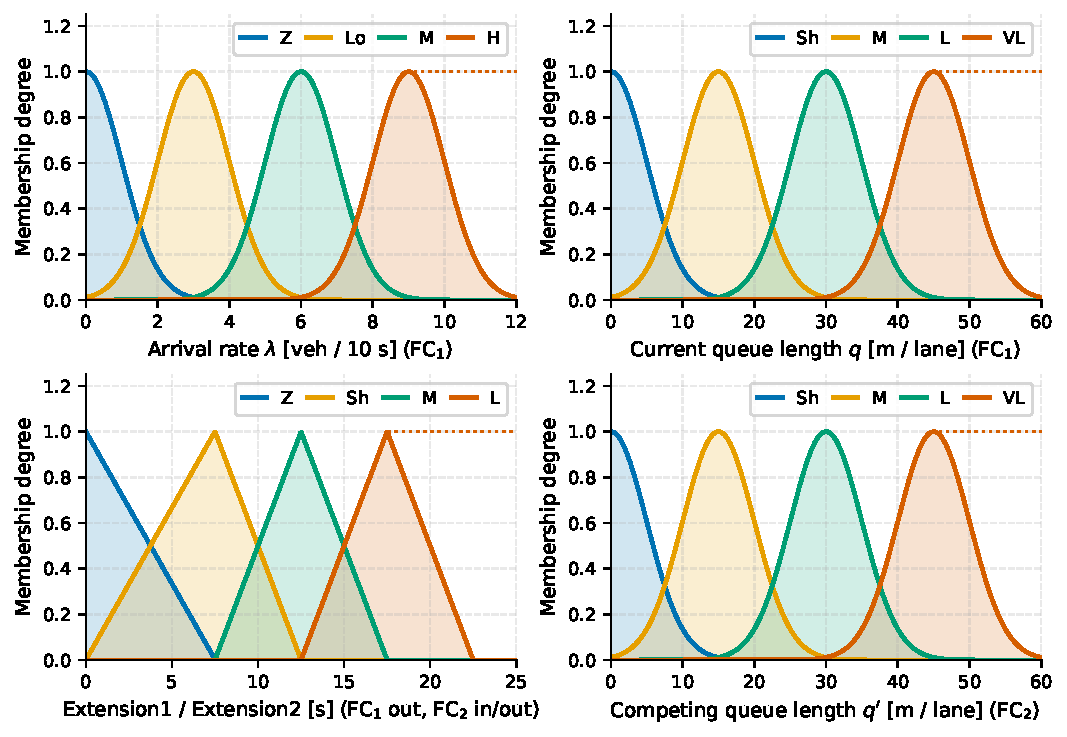
\includegraphics[width=0.82\textwidth]{fig/mf_inputs_outputs.pdf}
\caption{Yeniden gerçekleştirilen üyelik fonksiyonları: varış hızı ve mevcut kuyruk (FC$_1$ girişleri), Uzatma$_1$/Uzatma$_2$ ve rakip kuyruk (FC$_2$). Noktalı çizgiler omuz uzantılarıdır.}
\label{fig:mf}
\end{figure}

\textbf{Kural tabanlarının tamamlanması.} Makalede verilen 6 kuralı birebir sağlayan monoton bir tasarım kullanılmıştır. FC$_1$ için $\lambda$ ve kuyruk terimleri $0..3$ indeksleriyle kodlanmış ve Uzatma$_1=\lfloor(a+q)/2\rfloor$ alınmıştır (16 kural). FC$_2$ için rakip kuyruk cezası \{K:0, O:0, U:1, ÇU:2\} tanımlanmış ve Uzatma$_2=\max(0,e-\text{ceza})$ alınmıştır. $e=$Z olan dört kural tek kurala indiğinden tam olarak 13 kural elde edilir (Tablo~\ref{tab:rules}).

\begin{table}[t]
\centering
\caption{Tamamlanan kural tabanları. Kalın hücreler makalede birebir verilen kurallardır. Z: sıfır, K: kısa, O: orta, U: uzun, ÇU: çok uzun; Dü: düşük, Y: yüksek.}
\label{tab:rules}
\small
\begin{tabular}{@{}l|cccc@{}}
\toprule
\multicolumn{5}{c}{FC$_1$: Uzatma$_1$} \\
$\lambda\backslash q$ & K & O & U & ÇU \\
\midrule
Z & \textbf{Z} & Z & K & K \\
Dü & Z & K & \textbf{K} & O \\
O & \textbf{K} & K & O & O \\
Y & K & O & O & U \\
\bottomrule
\end{tabular}
\qquad
\begin{tabular}{@{}l|cccc@{}}
\toprule
\multicolumn{5}{c}{FC$_2$: Uzatma$_2$} \\
Uzatma$_1\backslash q'$ & K & O & U & ÇU \\
\midrule
Z & \multicolumn{4}{c}{\textbf{Z} (tek kural)} \\
K & K & \textbf{K} & Z & Z \\
O & \textbf{O} & O & K & Z \\
U & U & U & O & K \\
\bottomrule
\end{tabular}
\end{table}

\textbf{Çıkarım motorları.} Tüm motorlar aynı üyelik fonksiyonlarını ve kuralları kullanır:
\begin{itemize}
\item \emph{Mamdani}: min-VE, min-implikasyon, max-birleştirme ve 0,05 s ızgarada centroid.
\item \emph{Sugeno}: min-VE; sonuç sabitleri $\{0;7,5;12,5;17,5\}$ s olan sıfırıncı derece TSK.
\item \emph{OSFI-literal}: makalede yazıldığı gibi Łukasiewicz-VE ile ağırlıklı ortalama.
\item \emph{OSFI-DJ}: denklem~\eqref{eq:osfi}'in $d_1$ benzerliği ve Łukasiewicz implikatörüyle sayısal çözümü. $d_1$ hedefi $y$ üzerinde ayrıştığından her $y$ için $b\in[0,1]$ üzerinde 201 noktalı tek boyutlu bir arama yapılır; eşitlikte en küçük çözüm seçilir. Kurallar FITA yaklaşımıyla tek tek çıkarılıp gerçek implikatörler için minimumla birleştirilir. Implikatif çıktılar $(1-\alpha)$ tabanı taşıdığından taban çıkarılmış centroid kullanılır.
\item \emph{CRI}: aynı implikatörle sup-$T_\Luk$ kompozisyonu.
\end{itemize}
OSFI-DJ ve CRI için çevrimdışı arama tabloları (LUT) hesaplanmış, çalışma anında iki doğrusal ara değerleme kullanılmıştır.

\textbf{Faz geçiş mantığı ve ölü bölge yedeği.} Minimum yeşil (7 s) ve her uzatma penceresinin sonunda GPE çalıştırılır. Uzatma$_2\ge1$ s ise, mevcut kuyruk boş değilse ve yeşil 60 s'yi aşmamışsa yeşil uzatılır, aksi halde NPS'nin seçtiği faza geçilir. Bu yorum, makalenin ``GPE süreyi, NPS sıradaki fazı belirler'' tarifine dayanır. Diğer kuyruk daha uzun olduğu anda fazı kesen alternatif okuma (\texttt{preempt}) ablasyonda incelenmiştir (Bölüm~\ref{sec:res-abl}). Łukasiewicz VE işleminde tüm kuralların ateşleme gücü sıfırsa (ölü bölge), OSFI-literal, OSFI-DJ ve CRI motorlarında ortak bir ``en yakın kural'' yedeği uygulanır: min-ateşlemesi en büyük kuralın sonuç tepe değeri kullanılır.

\textbf{Karşılaştırma yöntemleri ve talep kalibrasyonu.} Webster sabit zamanlı planı~\cite{webster1958} gerçek ortalama talepten, durma çizgisi algılamalı araç uyarmalı kontrolcü ise 3 s birim uzatmayla hesaplanmıştır. Makale talep düzeyini vermediğinden, Tablo 1'deki Mamdani çıkışlarının toplamı (1064 araç) ve kuyruk evreninin 0--60 m (şerit başına $\approx$8,6 araç) olması esas alınmıştır. Yön dağılımı aynı tablodan (D 0,307; G 0,373; B 0,155; K 0,162) türetilmiştir.

\section{Önerilen Genişletme}
\label{sec:ext}

\subsection{Tekil girişte OSFI ile CRI denkliği}
\label{sec:prop}

\begin{proposition}
\label{prop:eq}
$A^*$, $x_0$ noktasında tekil bir küme olsun ve $I$ implikatörü $I(0,b)=1$ ile $I(1,b)=b$ koşullarını sağlasın (Łukasiewicz, Goguen, Kleene--Dienes). Bu durumda $d_1$ benzerliğiyle tanımlanan OSFI çözümü tektir ve
\begin{equation}
B^*(y)=I\big(A(x_0),B(y)\big)
\end{equation}
olur. Bu sonuç, aynı implikatörle CRI'nın verdiği sonuçla özdeştir.
\end{proposition}
\begin{proof}
$d_1$ hedefi $y$ üzerinde ayrışır: her $y$ için $\min_{b}\sum_x|I(A(x),B(y))-I(A^*(x),b)|$ çözülür. $x\neq x_0$ için $A^*(x)=0$ olduğundan $I(0,b)=1$ olur ve bu terimler $b$'den bağımsızdır. Geriye kalan tek terim $|I(A(x_0),B(y))-I(1,b)|=|I(A(x_0),B(y))-b|$'dir ve $b=I(A(x_0),B(y))$ noktasında tek biçimde sıfırlanır. CRI'da ise $\sup_xT(A^*(x),R(x,y))=R(x_0,y)=I(A(x_0),B(y))$ elde edilir.
\end{proof}
Mamdani'nin min işlemi $I(0,b)=0$ verdiğinden bu durumda çözüm $\min(A(x_0),B(y))$, yani Mamdani kırpmasıdır. Önermenin pratik sonucu şudur: tekil girişli bir kontrolcüde ``OSFI'' ile Mamdani arasındaki tüm farklar, benzerlik optimizasyonundan değil implikatör, birleştirme ve durulaştırma seçimlerinden kaynaklanır. Benzerlik optimizasyonu ancak giriş tekil değilse farklı bir sonuç üretebilir.

\subsection{Gürültüye dayanıklı non-singleton OSFI}

Referans makale, hatalı veya yetersiz sensörleri bir sınırlılık olarak belirtmektedir~\cite{esmaeili2025osfi}. Önerme~\ref{prop:eq} ile birlikte bu durum, OSFI'nin kendine özgü katkısını ortaya çıkarabileceği doğal bir ortam sunmaktadır. Önerilen \osfins{} kontrolcüsünde gürültülü ölçümler, merkezi ölçüm değeri olan Gauss kümelerle bulanıklaştırılır: $A^*(x_1,x_2)=A_1^*(x_1)A_2^*(x_2)$. Genişlikler sensör gürültüsüyle eşleştirilir: kuyruk için $\sigma_2=\max(\sigma_q,1)$ m, varış sayımı için kaçırma olasılığı $p$ olan binom inceltmenin ve yanlış sayımların varyansından $\sigma_1=\sqrt{0{,}5^2+2p(1-p)+0{,}2\,\mathbb{1}_{p>0}}$. Sonuç, denklem~\eqref{eq:osfi} doğrudan çözülerek elde edilir. Katkının kaynağını ayrıştırmak için iki kontrol koşulu tanımlanmıştır:
\begin{itemize}
\item \emph{CRI-NS}: aynı non-singleton girişlerle sup-T kompozisyonu. OSFI-NS ile CRI-NS arasındaki fark, yalnızca benzerlik optimizasyonunun etkisidir.
\item \emph{OSFI-DJ-NS-mis}: gerçek gürültüden bağımsız olarak $\sigma_2=5$ m sabit tutulur. Bu koşul, gürültü düzeyinin yanlış tahmin edilmesine karşı dayanıklılığı ölçer.
\end{itemize}

Gürültü modeli şöyledir: kuyruk ölçümü $\hat q=\max(0,q+\mathcal N(0,\sigma_q^2))$ ve $\sigma_q\in\{0,5,10,15\}$ m. Varış sayacı her aracı $1-p$ olasılıkla algılar ($p\in\{0;0{,}1;0{,}2\}$) ve $p>0$ iken 0,02 araç/s hızında yanlış sayım ekler. Gürültü akışları da tüm kontrolcüler için ortaktır. Şekil~\ref{fig:infex}, tek bir kural ve ölçüm için tekil OSFI, non-singleton CRI ve non-singleton OSFI sonuçlarının nasıl ayrıştığını göstermektedir.

\begin{figure}[t]
\centering
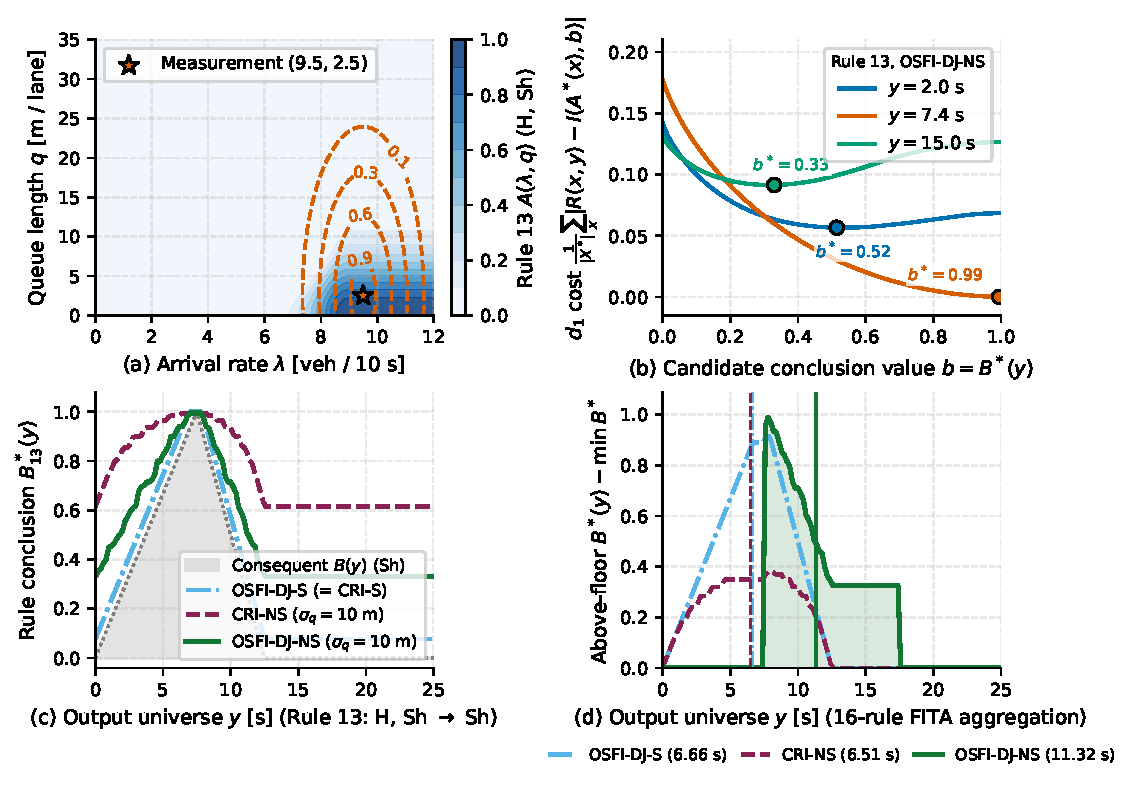
\includegraphics[width=0.86\textwidth]{fig/osfi_inference_example.pdf}
\caption{Bir çıkarım örneği ($\lambda=9{,}5$, $q=2{,}5$ m). (a) Kural 13'ün öncülü ve non-singleton giriş kümesi ($\sigma_q=10$ m). (b) Üç $y$ değeri için $d_1$ maliyeti ve en iyi $b$. (c) Kural sonucu: tekil OSFI, CRI ile çakışır (Önerme~\ref{prop:eq}); non-singleton girişte OSFI ile CRI ayrışır. (d) 16 kuralın birleşimi ve durulaştırılmış çıkışlar.}
\label{fig:infex}
\end{figure}

\section{Deneysel Kurulum}
\label{sec:setup}

Tablo~\ref{tab:setup} deney parametrelerini özetlemektedir. Dört senaryo kullanılmıştır: \emph{orta} (1100 araç/sa), \emph{ağır} (1500 araç/sa), \emph{tepe} (1100$\to$1800$\to$1100 araç/sa, 15 dk rampa ve 30 dk plato) ve doyma davranışını gözlemek için \emph{stres} (1800 araç/sa). Her koşul 30 ortak tohumla, 600 s ısınma ve 3600 s ölçüm süresiyle koşturulmuştur.

Ölçütler şunlardır: ayrılan araçların ortalama gecikmesi (s/araç), ölçüm penceresindeki araç çıkışı (veriş), ortalama kuyruk (m/şerit), faz değişim sayısı ve ölü bölge yedeği oranı. Ortalamalar \%95 $t$-güven aralığıyla (GA) verilmiştir. Eşleştirilmiş karşılaştırmalarda Wilcoxon işaretli sıra testi~\cite{wilcoxon1945} ve Holm düzeltmesi~\cite{holm1979} ($\alpha=0{,}05$) kullanılmıştır. Her koşuda iki doğrulama kapısı uygulanmıştır: aşırı doygun olmayan senaryolarda en az bir bulanık kontrolcü ile Webster, varışların en az \%97'sini boşaltmalı; kuyruk girişi en az üç dilsel kümede \%5'ten fazla bulunmalı. Bu kapıların ikisi de geçilmiştir.

Yazılım ortamı Python, NumPy 2.5.4, SciPy 1.18.1, pandas 3.1.1 ve Matplotlib 3.11.2'dir. Bulanık işleçlerin tamamı harici bir bulanık mantık kütüphanesi kullanılmadan yazılmıştır ve 30 test fonksiyonundan oluşan birim test paketiyle doğrulanmıştır. Deneyler Ubuntu 24.04 üzerinde çok çekirdekli paralel yürütülmüştür. Tüm katkı deneyleri (A, B, C; yaklaşık 7600 koşu) toplam 165 s sürmüştür.

\begin{table}[t]
\centering
\caption{Deney parametreleri.}
\label{tab:setup}
\small
\begin{tabular}{@{}ll@{}}
\toprule
Parametre & Değer \\
\midrule
Yaklaşım / şerit & 4 yaklaşım, yaklaşım başına 2 şerit, tek fazda tek yaklaşım \\
Servis & Üstel, 0,5 araç/s/şerit; kalkış kaybı 2 s; sarı 3 s + tüm-kırmızı 2 s \\
Yeşil sınırları & $G_{\min}=7$ s, $G_{\max}=60$ s \\
Sensör & Kuyruk: m/şerit (7 m/araç); varış: son 10 s'deki sayım \\
Süre / tekrar & 600 s ısınma + 3600 s ölçüm; 30 ortak tohum \\
Kontrolcüler & Mamdani, Sugeno, OSFI-literal, \osfis, CRI-S/NS, \osfins(-mis), Webster, Uyarmalı \\
Gürültü ızgarası & $\sigma_q\in\{0,5,10,15\}$ m $\times$ $p\in\{0;0{,}1;0{,}2\}$ (ağır ve tepe senaryoları) \\
OSFI-DJ ızgarası & $x_1,x_2$: 61 nokta; $y$: 0,2 s adım; $b$: 201 nokta; LUT ile ara değerleme \\
\bottomrule
\end{tabular}
\end{table}

\section{Sonuçlar}
\label{sec:results}

\subsection{Yeniden gerçekleştirme}

Tablo~\ref{tab:repro}, gürültüsüz ortamda tüm kontrolcülerin ortalama gecikmelerini, Şekil~\ref{fig:box} ise tohum bazındaki dağılımları göstermektedir. Makalenin iddia ettiği sıralama (OSFI $<$ Sugeno $<$ Mamdani) makalede yazıldığı biçimdeki OSFI-literal için yeniden üretilememiştir. OSFI-literal, orta trafikte Mamdani'den \%17, ağır trafikte \%149 daha yüksek gecikme vermiştir ($p_{\text{Holm}}<10^{-7}$). Buna karşılık Deng--Jiang'a sadık \osfis{}, tüm senaryolarda en düşük gecikmeyi elde etmiş ve Mamdani'ye göre orta trafikte \%6,2, ağır trafikte \%5,9 iyileşme sağlamıştır. Yani makalenin ``OSFI Mamdani'den daha iyidir'' yönündeki ana iddiası, yöntemin kuramsal tanımı uygulandığında desteklenmekte, ancak makalede yazılan formül uygulandığında desteklenmemektedir. Webster, tüm senaryolarda uyarlamalı kontrolcülerin gerisinde kalmıştır.

Tepe ve stres senaryolarında Sugeno ve OSFI-literal çökmüştür. Bu senaryolarda gecikme 190--390 s/araç, boşaltma oranı \%83--91 olmuştur. Kuyruklar 60 m'yi aştığında FC$_2$'deki rakip kuyruk cezası, ağırlıklı ortalamalı motorlarda uzatmayı neredeyse sıfırlamaktadır. Bu durumda kontrolcü her minimum yeşilden sonra faz değiştirir ve kayıp süre kapasiteyi tüketir. Centroid tabanlı Mamdani ve implikatif OSFI-DJ ise aynı kural tabanıyla daha geniş uzatma üretip doymadan uzak kalmıştır.

\begin{table}[t]
\centering
\caption{Gürültüsüz ortamda genel ortalama gecikme (s/araç, ortalama $\pm$ \%95 GA, $n=30$). Parantez içinde boşaltma oranı (\%). En iyi değerler kalındır. \osfis{} ve CRI-S tüm tohumlarda özdeştir.}
\label{tab:repro}
\small
\begin{tabular}{@{}lcccc@{}}
\toprule
Kontrolcü & Orta (1100) & Ağır (1500) & Tepe (1100--1800) & Stres (1800) \\
\midrule
Mamdani & 21,13 $\pm$ 0,30 & 25,58 $\pm$ 0,29 & 27,72 $\pm$ 0,45 & 29,48 $\pm$ 0,36 \\
Sugeno & 21,51 $\pm$ 0,46 & 44,52 $\pm$ 12,79 & 192,97 $\pm$ 25,47 (91,4) & 366,76 $\pm$ 35,13 (83,7) \\
OSFI-literal & 24,75 $\pm$ 0,47 & 63,79 $\pm$ 16,59 & 219,23 $\pm$ 22,80 (90,5) & 390,92 $\pm$ 31,48 (83,4) \\
\osfis{} = CRI-S & \textbf{19,82 $\pm$ 0,29} & \textbf{24,07 $\pm$ 0,35} & \textbf{26,26 $\pm$ 0,42} & \textbf{27,94 $\pm$ 0,39} \\
Webster & 30,57 $\pm$ 0,57 & 37,69 $\pm$ 0,88 & 41,18 $\pm$ 1,03 & 43,06 $\pm$ 0,91 \\
Uyarmalı & 22,63 $\pm$ 0,29 & 26,91 $\pm$ 0,39 & 29,30 $\pm$ 0,44 & 31,25 $\pm$ 0,44 \\
\bottomrule
\end{tabular}
\end{table}

\begin{figure}[t]
\centering
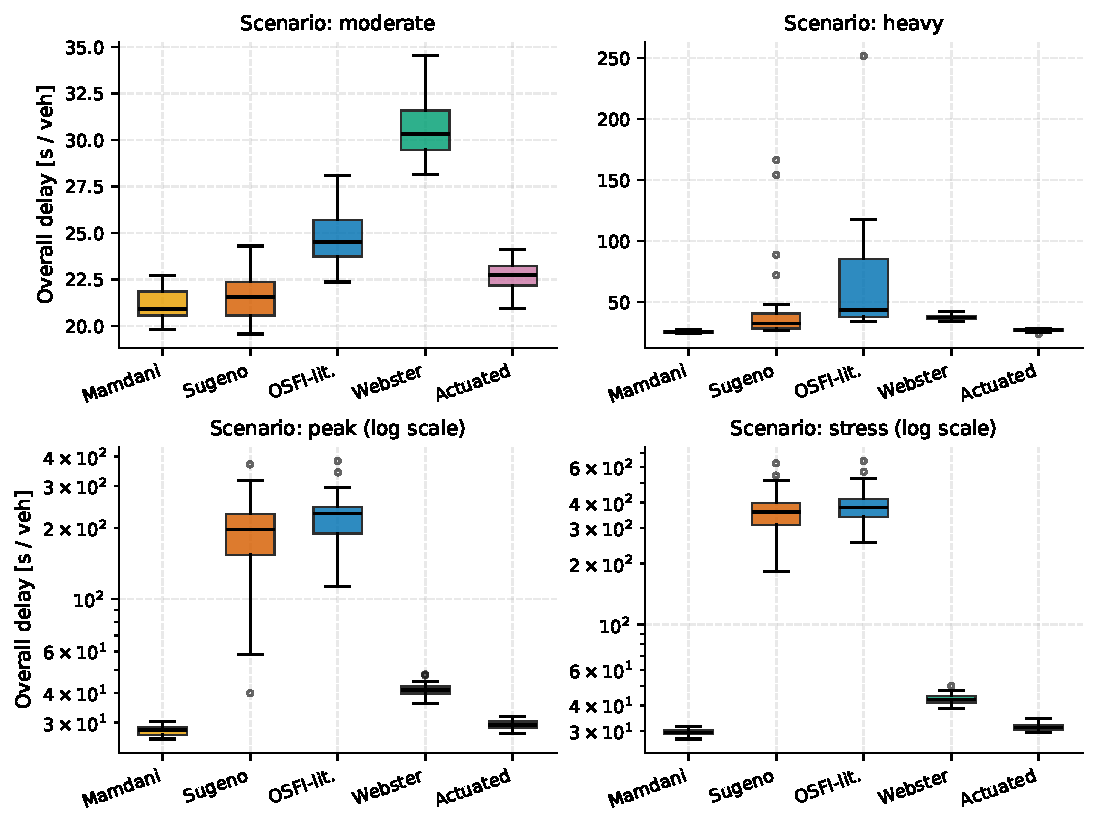
\includegraphics[width=0.78\textwidth]{fig/overall_delay_boxplot.pdf}
\caption{Tohum bazında genel gecikme dağılımları (30 tohum). Tepe ve stres senaryolarında y ekseni logaritmiktir; Sugeno ve OSFI-literal bu senaryolarda doymaktadır.}
\label{fig:box}
\end{figure}

Makaledeki Tablo 1--2 biçiminde yapılan faz bazında karşılaştırmada, araç çıkışları üç bulanık kontrolcüde \%1,5'ten daha az farklılaşmaktadır. Talep karşılandığı sürece çıkış, kontrolcüden çok talebe bağlıdır. Bu nedenle makalenin \%18,75'e varan ``çıkış iyileşmesi'' iddiası, hem işaret hatası (Bölüm~\ref{sec:original}) hem de bu fiziksel kısıt nedeniyle yeniden üretilememiştir.

\subsection{Önermenin deneysel doğrulanması}

Önerme~\ref{prop:eq} birim testlerinde ızgara noktalarında $<10^{-9}$ hata ile doğrulanmıştır. Simülasyonda da \osfis{} ve CRI-S dört senaryonun 120 koşusunun tamamında aynı faz kararlarını üretmiş ve birebir aynı metrikleri vermiştir (Tablo~\ref{tab:repro}). Mamdani ile aralarındaki \%5--6'lık fark, bu nedenle benzerlik optimizasyonundan değil, Łukasiewicz implikatörünün ve implikatif birleştirmenin daha geniş uzatma üretmesinden kaynaklanmaktadır (Şekil~\ref{fig:surf}).

\begin{figure}[t]
\centering
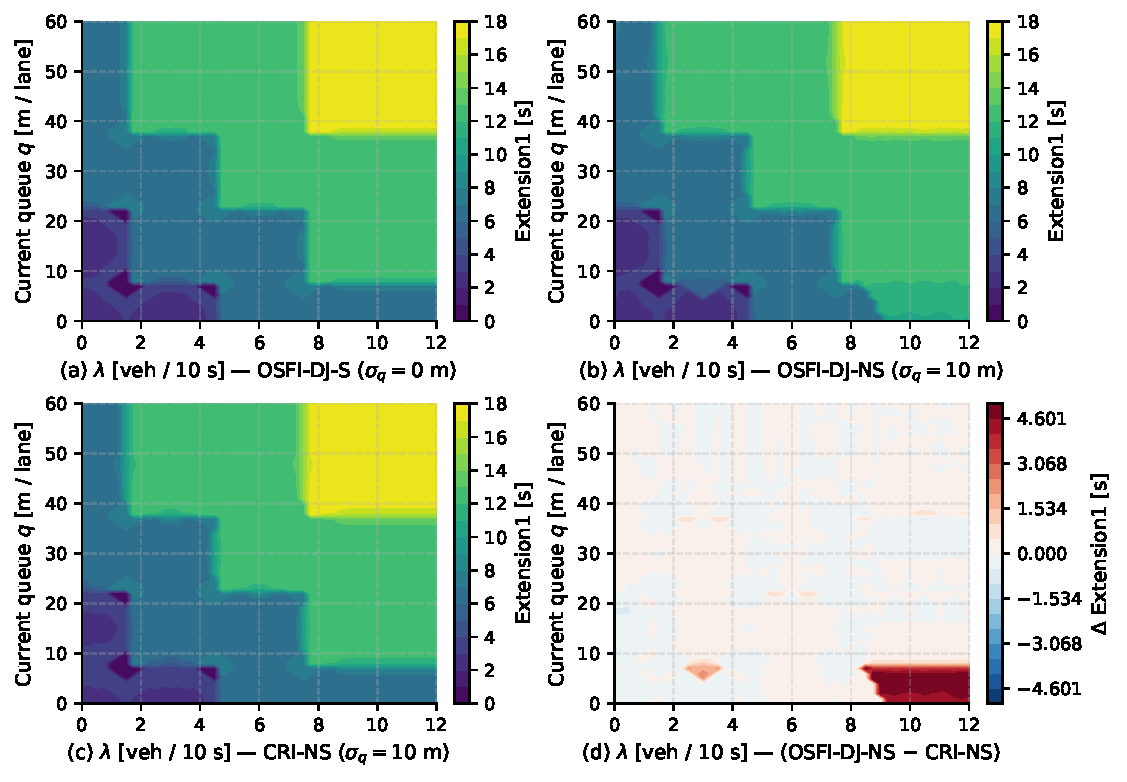
\includegraphics[width=0.92\textwidth]{fig/control_surfaces_osfi.pdf}
\caption{FC$_1$ kontrol yüzeyleri: (a) \osfis, (b) \osfins{} ($\sigma_q=10$ m), (c) CRI-NS, (d) \osfins{} $-$ CRI-NS farkı. Koyu karolar Łukasiewicz-VE ölü bölgeleridir (yedek kural devrededir).}
\label{fig:surf}
\end{figure}

\subsection{Sensör gürültüsü ve önerilen genişletme}

Gürültü, tüm uyarlamalı kontrolcüleri belirgin biçimde etkilemiştir (Şekil~\ref{fig:noise}). Ağır trafikte $\sigma_q$ 0'dan 15 m'ye çıktığında gecikme Mamdani'de \%46, \osfis{}'de \%52, Sugeno'da \%73 artmıştır. $\sigma_q=15$ m'de uyarlamalı kontrolcülerin üstünlüğü Webster'e karşı neredeyse kaybolmaktadır (36,2'ye karşı 37,7 s/araç). Varış sayacındaki kaçırmaların ($p$) etkisi, kuyruk gürültüsüne göre ikincil kalmıştır.

\begin{figure}[t]
\centering
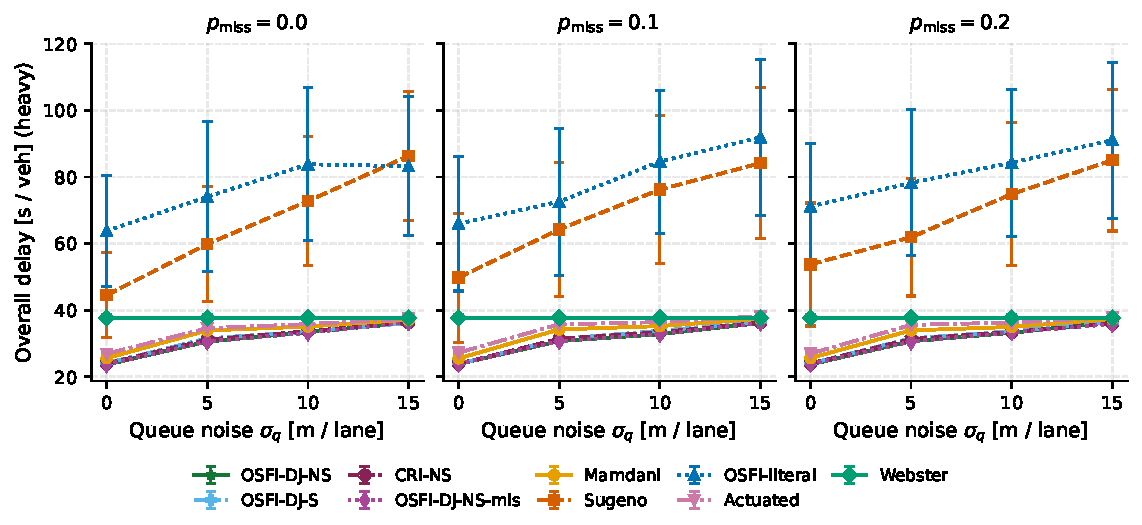
\includegraphics[width=\textwidth]{fig/noise_degradation_heavy.pdf}
\caption{Ağır senaryoda kuyruk sensörü gürültüsüne karşı genel gecikme (ortalama $\pm$ \%95 GA, $n=30$); paneller varış sayacı kaçırma olasılığına göredir.}
\label{fig:noise}
\end{figure}

Tablo~\ref{tab:contrib}, \osfis{} ile \osfins{} arasındaki karşılaştırmayı yönergenin istediği biçimde vermektedir. \osfins, 24 gürültü hücresinin 10'unda \osfis{}'ye göre, 9'unda ise CRI-NS'ye göre istatistiksel olarak anlamlı biçimde daha düşük gecikme vermiştir (Holm düzeltmeli Wilcoxon). Önerilen yöntemin anlamlı biçimde daha kötü olduğu hücre yoktur. İyileşme $\sigma_q=5$ m civarında yoğunlaşmaktadır: ağır senaryoda $p=0$ için medyan eşli fark $-1{,}28$ s/araç (\%$-4{,}1$), tepe senaryosunda $p=0{,}2$ için $-1{,}20$ s/araç (\%$-3{,}5$) olmuştur. $\sigma_q\ge10$ m'de farklar \%0--3 arasında kalmış ve çoğu hücrede anlamlı bulunmamıştır. Yanlış ayarlı genişlikle (\osfins-mis) elde edilen sonuçlar eşleştirilmiş sürümden ayırt edilememiştir. Bu durum, yöntemin gürültü düzeyinin tam bilinmesine duyarlı olmadığını göstermektedir. Önerilen yöntem, veriş ve kuyruk açısından tabanla eşdeğerdir. Hesaplama maliyeti ise doğrudan çıkarımda çağrı başına 1,3 ms'den 7,8 ms'ye çıkarken LUT ile $\approx$21 µs'de sabit kalmaktadır.

\begin{table}[t]
\centering
\caption{Yönerge §6.2 karşılaştırması: taban (\osfis) ve önerilen (\osfins). Gecikme s/araç, ortalama $\pm$ \%95 GA, $n=30$; $p$: varış kaçırma olasılığı.}
\label{tab:contrib}
\small
\begin{tabular}{@{}lccc@{}}
\toprule
Ölçüt (senaryo, gürültü) & \osfis & \osfins & Değişim \\
\midrule
Gecikme (ağır, $\sigma_q=0$, $p=0$) & 24,07 $\pm$ 0,35 & 23,67 $\pm$ 0,34 & $-$\%1,7 \\
Gecikme (ağır, $\sigma_q=5$, $p=0$) & 31,54 $\pm$ 0,46 & 30,59 $\pm$ 0,42 & $-$\%3,0 \\
Gecikme (ağır, $\sigma_q=10$, $p=0{,}1$) & 33,82 $\pm$ 0,47 & 32,80 $\pm$ 0,48 & $-$\%3,0 \\
Gecikme (ağır, $\sigma_q=15$, $p=0$) & 36,18 $\pm$ 0,54 & 36,18 $\pm$ 0,53 & \%0,0 \\
Gecikme (tepe, $\sigma_q=5$, $p=0$) & 33,80 $\pm$ 0,48 & 33,05 $\pm$ 0,60 & $-$\%2,2 \\
Gecikme (tepe, $\sigma_q=10$, $p=0$) & 35,77 $\pm$ 0,53 & 35,20 $\pm$ 0,65 & $-$\%1,6 \\
Veriş (ağır, $\sigma_q=10$; araç/sa) & 1501,7 $\pm$ 16,4 & 1500,6 $\pm$ 16,4 & $-$\%0,1 \\
Ortalama kuyruk (ağır, $\sigma_q=10$; m/şerit) & 12,33 $\pm$ 0,27 & 12,29 $\pm$ 0,29 & $-$\%0,3 \\
Çıkarım süresi, doğrudan (ms/çağrı) & 1,30 & 7,76 & $\times$6,0 \\
Çıkarım süresi, LUT (µs/çağrı) & 20,8 & 20,6 & $\approx$ \\
LUT hazırlama (FC$_1$+FC$_2$, s) & 0,92 & 3,92 & $+$3,0 s \\
\bottomrule
\end{tabular}
\end{table}

\subsection{Ablasyon ve ölü bölgeler}
\label{sec:res-abl}

Tablo~\ref{tab:abl}, ağır senaryoda $\sigma_q=10$ m için \osfins{} tasarım seçimlerinin etkisini göstermektedir. En büyük etki faz geçiş yorumundan gelmektedir. Rakip kuyruk daha uzun olduğu anda fazı kesen \texttt{preempt} okuma, gecikmeyi \%66 artırmakta ve faz değişimini saatte 194'ten 276'ya çıkarmaktadır. İkinci büyük etki durulaştırmadan gelmektedir: implikatif çıkışların $(1-\alpha)$ tabanı çıkarılmadan centroid alındığında uzatmalar orta değere doğru kaymakta ve gecikme \%48 artmaktadır. Goguen implikatörü Łukasiewicz'den biraz daha iyi sonuç vermiş (32,0 s), Kleene--Dienes ise yedek kural oranını \%28'e çıkarmıştır.

\begin{table}[t]
\centering
\caption{Ablasyon (ağır senaryo, $\sigma_q=10$ m, $p=0$, $n=30$). Taban: Łukasiewicz implikatörü, en küçük çözüm, taban çıkarılmış centroid, Łukasiewicz-VE, \texttt{gpe\_first}.}
\label{tab:abl}
\small
\begin{tabular}{@{}lccc@{}}
\toprule
Değişken & Gecikme (s/araç) & Faz değişimi/sa & Yedek oranı \\
\midrule
Taban (\osfins) & 33,44 $\pm$ 0,59 & 193,7 & \%2,6 \\
Goguen implikatörü & 32,04 $\pm$ 0,35 & 206,1 & \%1,0 \\
Kleene--Dienes implikatörü & 34,31 $\pm$ 0,59 & 216,8 & \%27,9 \\
Orta nokta eşitlik kuralı & 33,34 $\pm$ 0,46 & 194,0 & \%2,7 \\
Standart centroid (tabanlı) & 49,60 $\pm$ 0,75 & 110,0 & \%0,0 \\
Omuzsuz uç kümeler & 33,31 $\pm$ 0,50 & 194,5 & \%2,7 \\
min-VE & 33,88 $\pm$ 0,47 & 188,8 & \%0,0 \\
Üyelik genişliği $\times$1,5 & 32,90 $\pm$ 0,48 & 193,9 & \%0,0 \\
\texttt{preempt} faz geçişi & 55,54 $\pm$ 9,97 & 276,0 & \%2,9 \\
\bottomrule
\end{tabular}
\end{table}

Komşu Gauss kümeleri $\sigma_\lambda=1$, $\sigma_q=5$ ile $\approx0{,}32$ düzeyinde kesiştiğinden, kesişim noktalarının çevresinde her kural için $\mu_1+\mu_2-1\le0$ olur ve Łukasiewicz-VE hiçbir kuralı ateşlemez. Bu ölü bölgeler, FC$_1$ giriş düzleminin \%5'ini kaplar (Şekil~\ref{fig:dz}). Simülasyonda FC$_1$ değerlendirmelerinin \%2--8'i bu bölgelere düşmüştür. min-VE veya genişliği 1,5 kat artırılmış kümeler ölü bölgeyi tamamen kaldırmakta ve gecikmeyi değiştirmemekte ya da biraz iyileştirmektedir. Bu sonuç, makalenin Łukasiewicz-VE seçiminin üyelik fonksiyonlarıyla birlikte yeniden tasarlanması gerektiğini göstermektedir.

\begin{figure}[t]
\centering
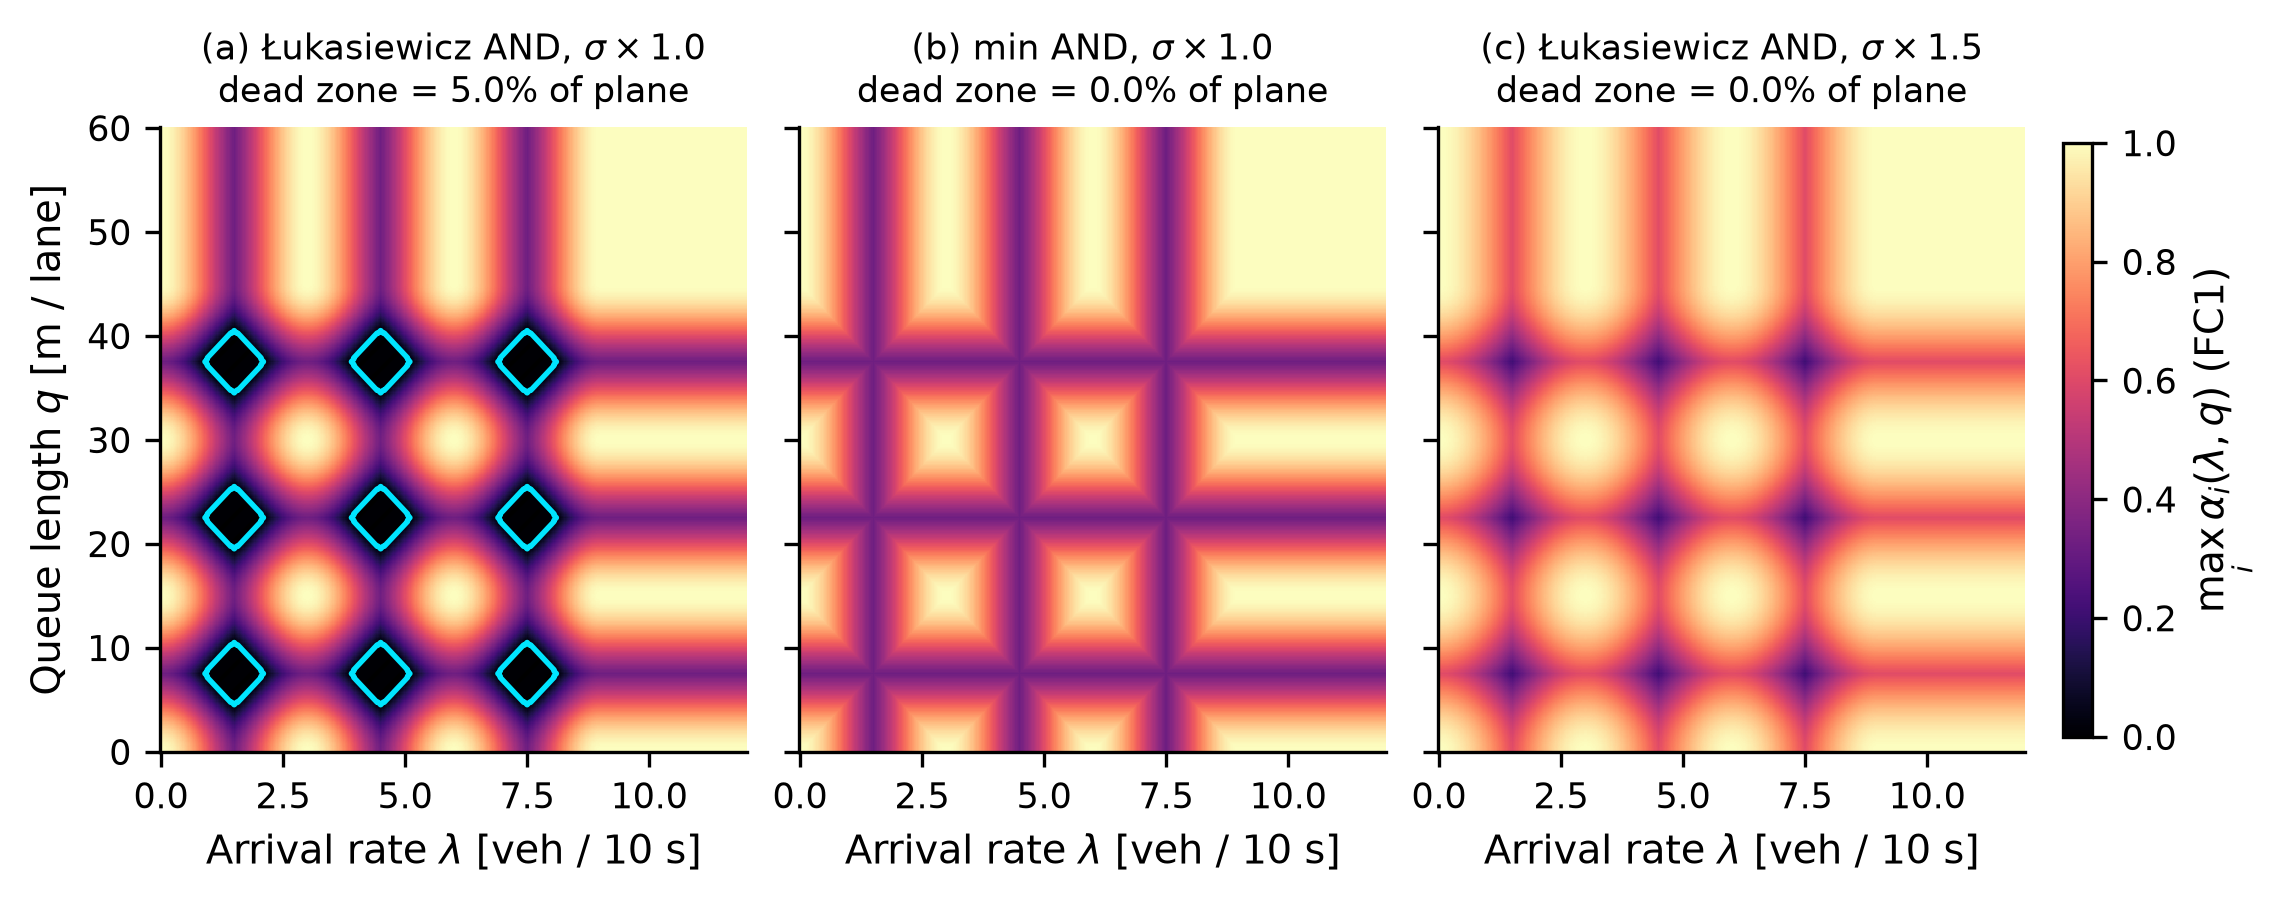
\includegraphics[width=0.92\textwidth]{fig/dead_zone_map.png}
\caption{FC$_1$'de en büyük kural ateşleme gücü $\max_i\alpha_i$: (a) Łukasiewicz-VE (ölü bölgeler turkuaz çerçeveli), (b) min-VE, (c) Łukasiewicz-VE ve 1,5 kat geniş Gauss kümeleri.}
\label{fig:dz}
\end{figure}

\section{Tartışma}
\label{sec:discussion}

Sonuçlar üç ana noktada toplanmaktadır. Birincisi, OSFI'nin bildirilen üstünlüğü yöntemin kuramsal tanımıyla tutarlıdır, ancak üstünlüğün kaynağı benzerlik optimizasyonu değildir. Önerme~\ref{prop:eq} ve özdeş simülasyon sonuçları, tekil girişli bir kontrolcüde OSFI'nin Łukasiewicz implikatörlü CRI ile aynı kararları verdiğini göstermektedir. Mamdani'ye göre kazanç, implikatif (``kural ihlal edildikçe sonuç gevşer'') yorumun ve taban çıkarılmış durulaştırmanın daha cömert yeşil uzatmalar üretmesinden gelmektedir. Makalede yazılan ağırlıklı ortalama formülü ise bu yapıyı kaybettiğinden Sugeno'ya benzer davranmakta ve doymaya yatkın hale gelmektedir.

İkincisi, benzerlik optimizasyonu non-singleton girişte gerçek bir fark yaratmaktadır. Ancak bu fark küçüktür ve gürültü arttıkça kaybolmaktadır. Orta gürültüde \osfins'in hem tekil OSFI'yi hem de aynı girişi kullanan CRI-NS'yi anlamlı biçimde geçmesi, iyileşmenin yalnızca girişi yumuşatmaktan değil, $d_1$ optimizasyonunun çıkış kümesini biçimlendirmesinden de kaynaklandığını göstermektedir. Yüksek gürültüde ($\sigma_q\ge10$ m, ortalama kuyruğun yaklaşık bir katı) ise ölçüm, giriş kümesi ne kadar iyi modellenirse modellensin bilgi taşımamaya başlar ve tüm uyarlamalı yöntemler Webster düzeyine yakınsar. Bu nedenle sahada, sensör iyileştirmesinin çıkarım tasarımından daha büyük etkisi olacağı beklenmelidir.

Üçüncüsü, kontrol mantığının ayrıntıları çıkarım motorundan daha belirleyicidir. Faz geçişi yorumu (\%66) ve durulaştırma tabanı (\%48), motorlar arasındaki farklardan (\%5--6) çok daha büyük etkiler yaratmıştır. Makalede bu ayrıntıların verilmemesi, raporlanan küçük yüzde farklarının (\%1--6) hangi tasarım seçimine ait olduğunun belirlenmesini olanaksız kılmaktadır.

\section{Sınırlılıklar}
\label{sec:limitations}

\begin{itemize}
\item Simülatör, makaleyle uyumlu bir kuyruk modelidir. Araç dinamiği, sol dönüşler, şerit değiştirme ve sürücü davranışı içermez. SUMO gibi mikroskobik bir simülatörde sonuçların büyüklüğü değişebilir.
\item Makalede eksik bırakılan 23 kural, üyelik parametreleri, talep düzeyleri ve faz geçiş mantığı varsayımla tamamlanmıştır. Farklı makul seçimler mutlak sayıları değiştirebilir. Bu nedenle değerlendirme göreli sıralamalara dayanmaktadır.
\item Gerçek dünya verisi kullanılmamıştır (makale de verisini tanımlamamaktadır). Talep, makalenin tablolarından kalibre edilmiş sentetik Poisson akışıdır.
\item Gürültü modeli bağımsız Gauss ve binom olarak tanımlanmıştır. Gerçek sensörlerde görülen ilişkili hatalar, sensör arızası ve kuyruğun algılama bölgesinin dışına taşması modellenmemiştir.
\item Çalışma tek bir izole kavşakla sınırlıdır. Kural tabanı ve üyelik fonksiyonları optimize edilmemiş, makaledekiler korunmuştur.
\item Önerilen yöntemin kazancı küçüktür (\%1--4) ve yüksek gürültüde kaybolmaktadır. LUT olmadan doğrudan çıkarım maliyeti yaklaşık 6 kat artmaktadır.
\end{itemize}

\section{Sonuç}
\label{sec:conclusion}

Bu projede OSFI tabanlı trafik sinyali kontrolcüsü açık ve test edilebilir bir biçimde yeniden gerçekleştirilmiş, referans makaledeki boşluklar ve tutarsızlıklar belgelenmiştir. Deng--Jiang tanımına sadık OSFI, Mamdani, Sugeno, Webster ve araç uyarmalı kontrolden daha düşük gecikme sağlamıştır. Bununla birlikte tekil girişte OSFI'nin CRI ile özdeş olduğu kuramsal ve deneysel olarak gösterilmiş, dolayısıyla kazancın kaynağının implikatör seçimi olduğu ortaya konmuştur. Önerilen non-singleton OSFI, düşük--orta sensör gürültüsünde istatistiksel olarak anlamlı ancak küçük bir ek iyileşme sağlamıştır. Ayrıca Łukasiewicz-VE ile makaledeki üyelik fonksiyonlarının ölü bölgeler oluşturduğu ve faz geçiş mantığının sonuçlara baskın etkisi olduğu gösterilmiştir.

Gelecek çalışmalar şunları içerebilir: (i) SUMO ile mikroskobik doğrulama ve gerçek kavşak verisi kullanımı, (ii) üyelik fonksiyonları ile kural tabanının ölü bölge kısıtı altında birlikte optimize edilmesi, (iii) sensör belirsizliğini doğrudan modelleyen aralık Tip-2 veya non-singleton Tip-2 varyantları, (iv) birden çok kavşağa genişletme.

\section*{Üretken Yapay Zekâ Kullanım Beyanı (Generative AI Usage Disclosure)}

Bu projede Anthropic'in Claude modeli (Claude Code ve Claude sohbet arayüzü üzerinden) yardımcı araç olarak kullanılmıştır. Kullanım alanları şunlardır: referans makaledeki eksik ve tutarsız noktaların listelenmesine yardım, Python kodunun ve birim testlerinin yazılması ve hata ayıklama, deney betiklerinin ve grafiklerin hazırlanması, literatür taramasında kaynak bulma ve raporun dil düzenlemesi. Önerme~\ref{prop:eq}'in türetimi, simülasyon sonuçları ve istatistiksel analizler öğrenci tarafından kod ve testler üzerinden kontrol edilmiştir. Kaynakçadaki tüm çalışmalar referans makalenin kaynakçasından veya yayıncı/DOI kayıtlarından doğrulanmıştır. Sonuçların ve yorumların sorumluluğu öğrenciye aittir.

\bibliographystyle{ieeetr}
\bibliography{references}

\end{document}
